\chapter{Analyse de l'existant}

WabinPaint est un logiciel utilisant la librairie Clutter. Voici un descriptif plus technique de WabinPaint, ce qui permettra de modéliser une solution pour l'implémentation de la Kinect.

\section{Clutter}

	Clutter est une bibliothèque logicielle permettant la création rapide d'interfaces graphiques visuellement riches et animées. C'est un projet libre (licence GNU LGPL) et multiplate-forme. Clutter est basée sur glib, librairie de l'écosystème Gnome.
	
	Clutter ne gère en périphérique d'entrée que la souris. Cependant il est possible d'associer des données (avec Kinect, la position des mains) à la structure de données représentant la souris. WabinPaint possède déjà une classe qui permettra à notre implémentation Kinect de faire ces opérations, de convertir les positions en événement souris. Cette classe se nomme GenericTracker et est déjà utilisé par les trackers "réels" ART et Vicon. Son utilisation sera détaille dans le chapitre Kinect.
	
\section{Choix techniques}

	OpenNI est une librairie permettant de récupérer la position des mains. Une description de OpenNI plus approfondie est disponible dans le chapitre Kinect.
	
	Pour fonctionner OpenNI nécessite de créer une boucle de traitement pour continuellement fournir la position des mains. Pour cette raison et pour ne pas bloquer la boucle de la glib, il est nécessaire d'éxécuter OpenNI dans un thread différent.
	
	À ce problème s'offre deux possibilités, utiliser un thread glib, ou utiliser une application externe (un serveur) et intégrer une partie client en utilisant
     une fonction "idle" dans WabinPaint. C'est cette 2\up{ème} solution qui
     a été choisie pour les deux trackers déjà implémentés dans WabinPaint. L'implémentation de la Kinect sera similaire.
     
 \section{Mise en œuvre}

Pour nous aider au maximum à identifier les différentes parties du projet, nous avons défini plusieurs briques (composantes) visibles ci-dessous:

\begin{figure}[!ht]
	\center
	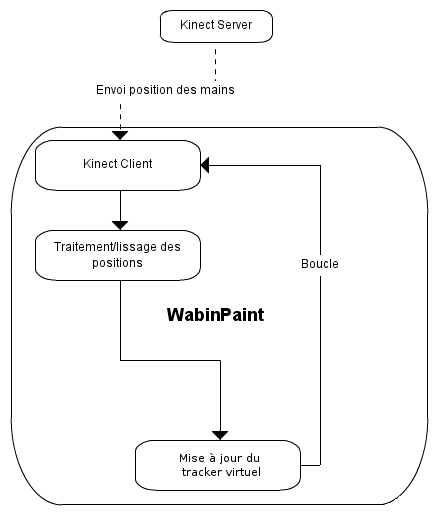
\includegraphics[scale=0.5]{image/plan.png}
	\caption{Composantes à réaliser}
\end{figure}

Sur ce schéma nous retrouvons l'ensemble des éléments nécessaires pour remplir les objectifs de notre projet, une acquisition via Kinect, un traitement des données et finalement envoyer les informations à d'autre composantes de WabinPaint pour permettre la mise à jour du canvas.

Le projet sera réalisé en C++, comme WabinPaint, et nous aurons à utiliser les librairies (OpenNI) fournies par PrimeSense pour l'utilisation de la Kinect sous Linux, de OSC, une librairie nous permettant de faire la liaison entre serveur et client ainsi que des algorithmes de traitement de données tels que l'algorithme nommé \textit{One Euro Filter}.

